\documentclass[12pt]{article}
\usepackage{graphicx}
\usepackage{tikz}
\graphicspath{ {./images/} }

\title{Limit Order Token Reserves - Tokenized Exchange Orders as Hedging Vehicles}
\author{Sean Hart}

\begin{document}
   \maketitle

   \begin{abstract}

   \end{abstract}

   \section*{Introduction}
   The advent of programmable decentralized ledgers have introduced the ability to create highly complex fungible structured products that can exist independently from their issuing organization. This contract independence allows for the creation of products with direct ownership of embedded collateral that do not require the continued existence of a solvent external entity in an enforceable jurisdiction. This unique feature combination in addition to the rise of decentralized exchanges allows for the creation of previously impossible product types, such as encapsulated and fungible pending exchange orders that automatically execute when specific criteria are reached.

   Specifically, Limit Order Token Reserve (LOTR) tokens are Tokenized (encapsulated and fungible) Exchange Orders with embedded collateral used for exchange payment when the targeted asset is confirmed to have reached the limit price on a decentralized exchange. Minters of LOTRs receive two tokens, one Limit Order token representing the receiver of the target token when the limit price is reached, and one Redeem Token required to unlock the embedded collateral in the limit order \$Tokent any time before the target token limit price is reached. Both of these tokens are fungible, meaning that they can be paired with any opposing LOTR token, and therefore tradable on secondary markets. This secondary market composability allows this product to be used as a hedging or speculative vehicle, with owners selling one half of the LOTR token pair with the expectation of their half diverging in market price from their purchase price when the underlying asset price changes relative to the LOTR limit order price. The LOTR token pair halves always sum to the limit order price (the value of redeemable embedded collateral) minus transfer fees.

   Traders will find that the value of LOTR tokens is easier to calculate than perpetual options because they automatically execute when the asset reaches the limit order price, removing the unlimited best price problem. This automatic execution means LOTR tokens are therefore not "options". LOTRs are also more fungible than expiring options because LOTR products have one fewer variable (expiration date). Closer examination will also reveal behavioral similarities with futures contracts due to the product valuation being equal to the underlying asset price and without the requirement for a product premium payment as with options contracts.

   \section*{Usage}
      \subsection*{Minting}
         To be used as hedging or speculative vehicles, LOTR tokens must have a minting process that does not affect their price on the open market. Fortunately, LOTR token pairs always sum to the value of embedded collateral in the token, which is also the target price for the limit order. Therefore, any entity can set up a token smart contract that issues the LOTR token pairs and stores the ownership balances on an embedded ledger.
         % MINTING GRAPHIC
         \begin{center}
            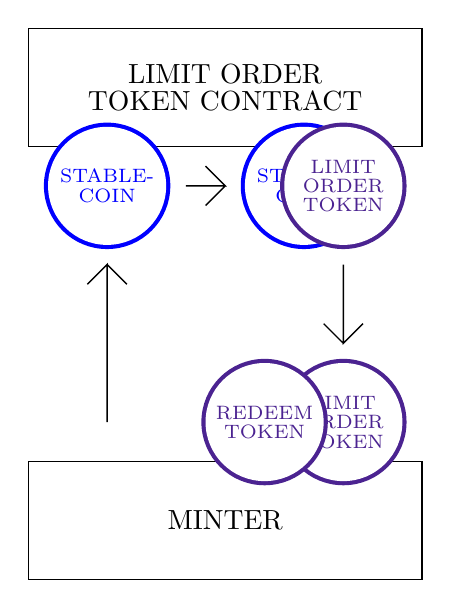
\begin{tikzpicture}
               % bottom box
               \draw [line width=0.5, black] (0,0) -- (5,0) -- (5,1.5) -- (0,1.5) -- (0,0);
               \node [align=center,font=\fontsize{10pt}{10pt}\selectfont] at (2.5,0.75) {MINTER};
               % arrow up
               \draw [line width=0.5, black] (1,2) -- (1,4) -- (0.75,3.75) -- (1,4) -- (1.25,3.75);
               % top box
               \draw [line width=0.5, black] (0,5.5) -- (5,5.5) -- (5,7) -- (0,7) -- (0,5.5);
               \node [align=center,font=\fontsize{10pt}{10pt}\selectfont] at (2.5,6.25) {LIMIT ORDER\\TOKEN CONTRACT};
               % STABLECOIN top left
               \draw [line width=3, blue] (1,5) circle (0.75);
               \fill [white,fill opacity=1] (1,5) circle (0.75);
               \node [color=blue,align=center,font=\fontsize{7pt}{7pt}\selectfont] at (1,5) {STABLE-\\COIN};
               % arrow right
               \draw [line width=0.5, black] (2,5) -- (2.5,5) -- (2.25,5.25) -- (2.5,5) -- (2.25,4.75);
               % STABLECOIN top right
               \draw [line width=3, blue] (3.5,5) circle (0.75);
               \fill [white,fill opacity=1] (3.5,5) circle (0.75);
               \node [color=blue,align=center,font=\fontsize{7pt}{7pt}\selectfont] at (3.5,5) {STABLE-\\COIN};
               % Limit Order Token top right
               \draw [line width=3, color={rgb:red,130;green,60;blue,250}] (4,5) circle (0.75);
               \fill [white,fill opacity=1] (4,5) circle (0.75);
               \node [color={rgb:red,130;green,60;blue,250},align=center,font=\fontsize{7pt}{7pt}\selectfont] at (4,5) {LIMIT\\ORDER\\TOKEN};
               % arrow down
               \draw [line width=0.5, black] (4,4) -- (4,3) -- (4.25,3.25) -- (4,3) -- (3.75,3.25);
               % Limit Order Token bottom right
               \draw [line width=3, color={rgb:red,130;green,60;blue,250}] (4,2) circle (0.75);
               \fill [white,fill opacity=1] (4,2) circle (0.75);
               \node [color={rgb:red,130;green,60;blue,250},align=center,font=\fontsize{7pt}{7pt}\selectfont] at (4,2) {LIMIT\\ORDER\\TOKEN};
               % Redeem Token bottom right
               \draw [line width=3, color={rgb:red,130;green,60;blue,250}] (3,2) circle (0.75);
               \fill [white,fill opacity=1] (3,2) circle (0.75);
               \node [color={rgb:red,130;green,60;blue,250},align=center,font=\fontsize{7pt}{7pt}\selectfont] at (3,2) {REDEEM\\TOKEN};
            \end{tikzpicture}
         \end{center}
         All tokens minted by the same contract are fungible since they share a ledger and handling functions.

      \subsection*{Trading}
         LOTR token contracts should be written in a chain-standardized format to allow composability across DeFi token protocols on the same chain. This composability allows for open market trading independent of the issuing contract. This feature is key to LOTR token halves use as hedging or speculative vehicles since token halves can be combined with various uncorrelated assets.
         % TRADING GRAPHIC
         \begin{center}
            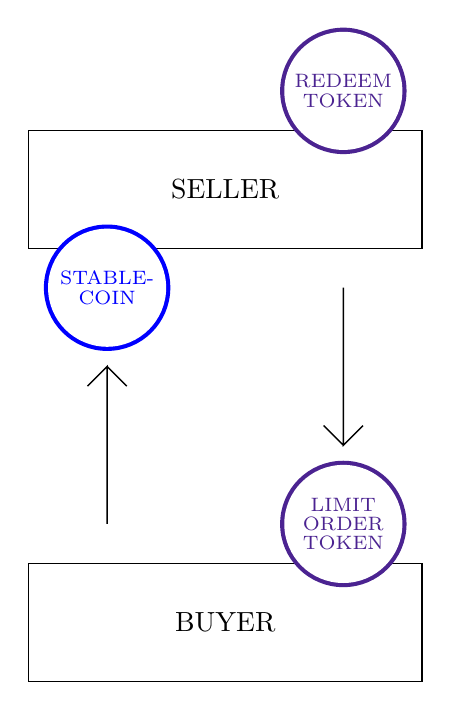
\begin{tikzpicture}
               % bottom box
               \draw [line width=0.5, black] (0,0) -- (5,0) -- (5,1.5) -- (0,1.5) -- (0,0);
               \node [align=center,font=\fontsize{10pt}{10pt}\selectfont] at (2.5,0.75) {BUYER};
               % arrow up
               \draw [line width=0.5, black] (1,2) -- (1,4) -- (0.75,3.75) -- (1,4) -- (1.25,3.75);
               % top box
               \draw [line width=0.5, black] (0,5.5) -- (5,5.5) -- (5,7) -- (0,7) -- (0,5.5);
               \node [align=center,font=\fontsize{10pt}{10pt}\selectfont] at (2.5,6.25) {SELLER};
               % STABLECOIN top left
               \draw [line width=3, blue] (1,5) circle (0.75);
               \fill [white,fill opacity=1] (1,5) circle (0.75);
               \node [color=blue,align=center,font=\fontsize{7pt}{7pt}\selectfont] at (1,5) {STABLE-\\COIN};
               % Redeem Token
               \draw [line width=3, color={rgb:red,130;green,60;blue,250}] (4,7.5) circle (0.75);
               \fill [white,fill opacity=1] (4,7.5) circle (0.75);
               \node [color={rgb:red,130;green,60;blue,250},align=center,font=\fontsize{7pt}{7pt}\selectfont] at (4,7.5) {REDEEM\\TOKEN};
               % arrow down
               \draw [line width=0.5, black] (4,5) -- (4,3) -- (4.25,3.25) -- (4,3) -- (3.75,3.25);
               % Limit Order Token bottom right
               \draw [line width=3, color={rgb:red,130;green,60;blue,250}] (4,2) circle (0.75);
               \fill [white,fill opacity=1] (4,2) circle (0.75);
               \node [color={rgb:red,130;green,60;blue,250},align=center,font=\fontsize{7pt}{7pt}\selectfont] at (4,2) {LIMIT\\ORDER\\TOKEN};
            \end{tikzpicture}
         \end{center}

      \subsection*{Outcomes}
         LOTR tokens have two possible outcomes: redemption of the embedded collateral or execution of the limit order. Both outcomes burn the expended tokens.
         \subsubsection*{Redemption}
            Any holder of both LOTR token halves can choose to redeem the embedded collateral, minus transfer fees, at any time. This process is initiated by passing the Redeem \$Tokenddress to a function on the Limit Order function. This process burns the two token halves involved in the redemption function and transfers the embedded collateral ownership to the final address of both LOTR token halves used (the ownership address of both token halves must be the same).
            % REDEEM GRAPHIC
            \begin{center}
               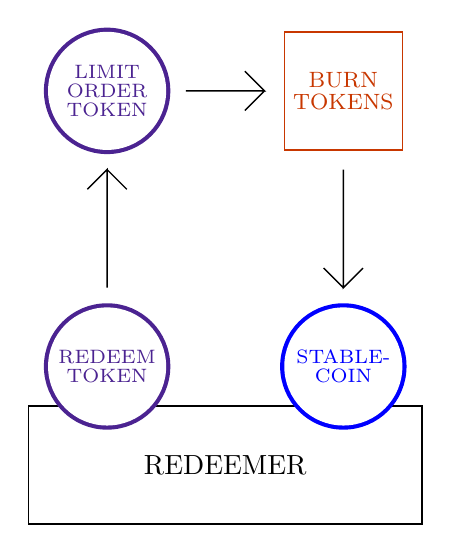
\begin{tikzpicture}
                  % bottom box
                  \draw [line width=0.5, black] (0,0) -- (5,0) -- (5,1.5) -- (0,1.5) -- (0,0);
                  \node [align=center,font=\fontsize{10pt}{10pt}\selectfont] at (2.5,0.75) {REDEEMER};
                  % Redeem Token bottom left
                  \draw [line width=3, color={rgb:red,130;green,60;blue,250}] (1,2) circle (0.75);
                  \fill [white,fill opacity=1] (1,2) circle (0.75);
                  \node [color={rgb:red,130;green,60;blue,250},align=center,font=\fontsize{7pt}{7pt}\selectfont] at (1,2) {REDEEM\\TOKEN};
                  % arrow up
                  \draw [line width=0.5, black] (1,3) -- (1,4.5) -- (0.75,4.25) -- (1,4.5) -- (1.25,4.25);
                  % Limit Order Token top left
                  \draw [line width=3, color={rgb:red,130;green,60;blue,250}] (1,5.5) circle (0.75);
                  \fill [white,fill opacity=1] (1,5.5) circle (0.75);
                  \node [color={rgb:red,130;green,60;blue,250},align=center,font=\fontsize{7pt}{7pt}\selectfont] at (1,5.5) {LIMIT\\ORDER\\TOKEN};
                  % arrow right
                  \draw [line width=0.5, black] (2,5.5) -- (3,5.5) -- (2.75,5.75) -- (3,5.5) -- (2.75,5.25);
                  % Burn tokens box
                  \draw [line width=0.5, color={rgb:red,255;green,70;blue,0}] (3.25,4.75) -- (3.25,6.25) -- (4.75,6.25) -- (4.75,4.75) -- (3.25,4.75);
                  \node [color={rgb:red,255;green,70;blue,0},align=center,font=\fontsize{8pt}{8pt}\selectfont] at (4,5.5) {BURN\\TOKENS};
                  % arrow down
                  \draw [line width=0.5, black] (4,4.5) -- (4,3) -- (4.25,3.25) -- (4,3) -- (3.75,3.25);
                  % STABLECOIN bottom right
                  \draw [line width=3, blue] (4,2) circle (0.75);
                  \fill [white,fill opacity=1] (4,2) circle (0.75);
                  \node [color=blue,align=center,font=\fontsize{7pt}{7pt}\selectfont] at (4,2) {STABLE-\\COIN};
               \end{tikzpicture}
            \end{center}

         \subsubsection*{Execution}
            The execution outcome is the most complicated function of the LOTR token contract. The end goal of this function is to transfer all embedded collateral to all owners of Limit Order tokens, and burn all Limit Order and Redeem Tokens for all current owners. When this function completes, all LOTR balances are zero and LOTR's balances on external token contracts (embedded collateral contracts) are also zero (it should not own any embedded collateral). This process resets the LOTR token so it can be used again until the execution function is called when the limit price is reached once again. This cycle repeats perpetually.

            The execution function can be engineered to be triggered in a variety of ways. Either a centralized entity can monitor the market and trigger the function when the limit price is reached, or a decentralized incentive process can be used to encourage any on-chain actor to call the execution function and be rewarded with a cut of fees if the limit price is confirmed to have been reached.
            % EXECUTION GRAPHIC
            \begin{center}
               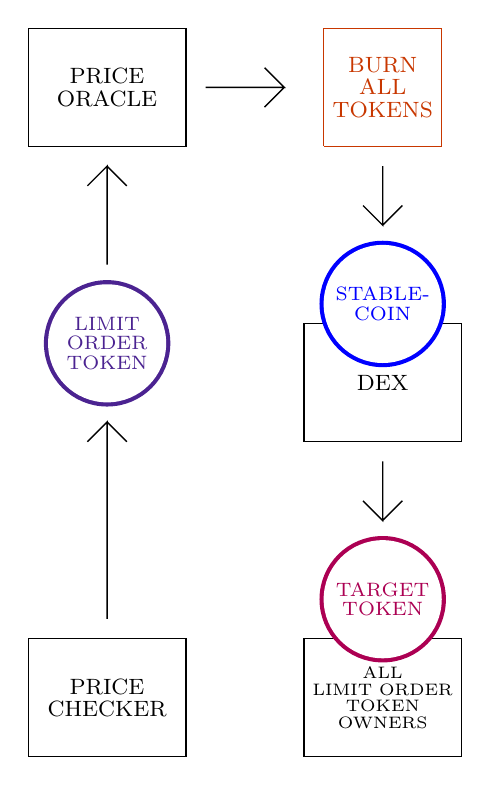
\begin{tikzpicture}
                  % bottom left box
                  \draw [line width=0.5, black] (0,0) -- (2,0) -- (2,1.5) -- (0,1.5) -- (0,0);
                  \node [align=center,font=\fontsize{8pt}{8pt}\selectfont] at (1,0.75) {PRICE\\CHECKER};
                  % arrow up
                  \draw [line width=0.5, black] (1,1.75) -- (1,4.25) -- (0.75,4) -- (1,4.25) -- (1.25,4);
                  % Limit Order Token left
                  \draw [line width=3, color={rgb:red,130;green,60;blue,250}] (1,5.25) circle (0.75);
                  \fill [white,fill opacity=1] (1,5.25) circle (0.75);
                  \node [color={rgb:red,130;green,60;blue,250},align=center,font=\fontsize{7pt}{7pt}\selectfont] at (1,5.25) {LIMIT\\ORDER\\TOKEN};
                  % arrow up
                  \draw [line width=0.5, black] (1,6.25) -- (1,7.5) -- (0.75,7.25) -- (1,7.5) -- (1.25,7.25);
                  % Oracle box
                  \draw [line width=0.5, black] (0,7.75) -- (2,7.75) -- (2,9.25) -- (0,9.25) -- (0,7.75);
                  \node [color=black,align=center,font=\fontsize{8pt}{8pt}\selectfont] at (1,8.5) {PRICE\\ORACLE};
                  % arrow right
                  \draw [line width=0.5, black] (2.25,8.5) -- (3.25,8.5) -- (3,8.75) -- (3.25,8.5) -- (3,8.25);
                  % Burn tokens box
                  \draw [line width=0.5, color={rgb:red,255;green,70;blue,0}] (3.75,7.75) -- (3.75,9.25) -- (5.25,9.25) -- (5.25,7.75) -- (3.75,7.75);
                  \node [color={rgb:red,255;green,70;blue,0},align=center,font=\fontsize{8pt}{8pt}\selectfont] at (4.5,8.5) {BURN\\ALL\\TOKENS};
                  % arrow down
                  \draw [line width=0.5, black] (4.5,7.5) -- (4.5,6.75) -- (4.25,7) -- (4.5,6.75) -- (4.75,7);
                  % DEX box
                  \draw [line width=0.5, color=black] (3.5,4) -- (3.5,5.5) -- (5.5,5.5) -- (5.5,4) -- (3.5,4);
                  \node [color=black,align=center,font=\fontsize{8pt}{8pt}\selectfont] at (4.5,4.75) {DEX};
                  % STABLECOIN
                  \draw [line width=3, blue] (4.5,5.75) circle (0.75);
                  \fill [white,fill opacity=1] (4.5,5.75) circle (0.75);
                  \node [color=blue,align=center,font=\fontsize{7pt}{7pt}\selectfont] at (4.5,5.75) {STABLE-\\COIN};
                  % arrow down
                  \draw [line width=0.5, black] (4.5,3.75) -- (4.5,3) -- (4.25,3.25) -- (4.5,3) -- (4.75,3.25);
                  % bottom right box
                  \draw [line width=0.5, black] (3.5,0) -- (5.5,0) -- (5.5,1.5) -- (3.5,1.5) -- (3.5,0);
                  \node [align=center,font=\fontsize{6pt}{6pt}\selectfont] at (4.5,0.75) {ALL\\LIMIT ORDER\\TOKEN\\OWNERS};
                  % Target Token
                  \draw [line width=3, color={rgb:red,255;green,0;blue,122}] (4.5,2) circle (0.75);
                  \fill [white,fill opacity=1] (4.5,2) circle (0.75);
                  \node [color={rgb:red,255;green,0;blue,122},align=center,font=\fontsize{7pt}{7pt}\selectfont] at (4.5,2) {TARGET\\TOKEN};
               \end{tikzpicture}
            \end{center}
            Certain advanced on-chain external contract calls are required in the execution function. First, the market price should be checked to ensure the limit price has been reached. This check should occur whether the execution function is triggered by a centralized entity or a decentralized on-chain actor. Ideally the oracle(s) used to check the market price use a variety of reporting sources to ensure accuracy. It is also recommended to use an oracle related to the exchange used in the swap process to ensure the swap occurs as close to the limit price as possible. Second, an exchange must be called to process the swap orders. Ideally the exchange is decentralized with enough liquidity to process the orders without significant price slippage.

            The use of external oracles and exchanges preset opportunities for transaction failure. The execution function should include appropriate fallback procedures. Some fallback options are centralized, such as the LOTR issuer manually retrying execution, but other options are more simple such as releasing the embedded funds to Limit Order token owners to allow them to manually attempt the token swap on their own terms. Depending on the complexity of other various setups of the LOTR contract, these necessary fallback procedures can be more or less complex.
            
            Once the limit price has been passed, the LOTR token contract should also track the new price direction of the current market (below or above the limit price). During the price check or use of a fallback procedure, the directionality is often needed to confirm the market price passed the limit price away from the previous price direction.

   \section*{Example}
      Consider an investor seeking to reduce the risk of an investment in \$Token. \$Token is currently trading at \$12 per token. The investor mints an LOTR token pair at the limit price of \$10, paying \$10 in equivalent tokens and receiving the token pair. Expense = \$10.
      % MINTING GRAPHIC
      \begin{center}
         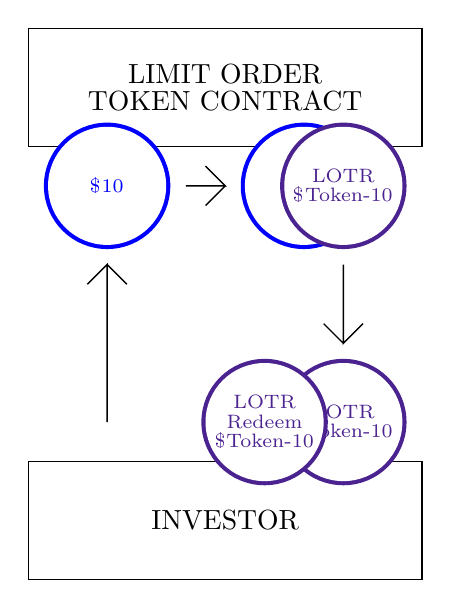
\begin{tikzpicture}
            % bottom box
            \draw [line width=0.5, black] (0,0) -- (5,0) -- (5,1.5) -- (0,1.5) -- (0,0);
            \node [align=center,font=\fontsize{10pt}{10pt}\selectfont] at (2.5,0.75) {INVESTOR};
            % arrow up
            \draw [line width=0.5, black] (1,2) -- (1,4) -- (0.75,3.75) -- (1,4) -- (1.25,3.75);
            % top box
            \draw [line width=0.5, black] (0,5.5) -- (5,5.5) -- (5,7) -- (0,7) -- (0,5.5);
            \node [align=center,font=\fontsize{10pt}{10pt}\selectfont] at (2.5,6.25) {LIMIT ORDER\\TOKEN CONTRACT};
            % STABLECOIN top left
            \draw [line width=3, blue] (1,5) circle (0.75);
            \fill [white,fill opacity=1] (1,5) circle (0.75);
            \node [color=blue,align=center,font=\fontsize{7pt}{7pt}\selectfont] at (1,5) {\$10};
            % arrow right
            \draw [line width=0.5, black] (2,5) -- (2.5,5) -- (2.25,5.25) -- (2.5,5) -- (2.25,4.75);
            % STABLECOIN top right
            \draw [line width=3, blue] (3.5,5) circle (0.75);
            \fill [white,fill opacity=1] (3.5,5) circle (0.75);
            \node [color=blue,align=center,font=\fontsize{7pt}{7pt}\selectfont] at (3.5,5) {\$10};
            % Limit Order Token top right
            \draw [line width=3, color={rgb:red,130;green,60;blue,250}] (4,5) circle (0.75);
            \fill [white,fill opacity=1] (4,5) circle (0.75);
            \node [color={rgb:red,130;green,60;blue,250},align=center,font=\fontsize{7pt}{7pt}\selectfont] at (4,5) {LOTR\\\$Token-10};
            % arrow down
            \draw [line width=0.5, black] (4,4) -- (4,3) -- (4.25,3.25) -- (4,3) -- (3.75,3.25);
            % Limit Order Token bottom right
            \draw [line width=3, color={rgb:red,130;green,60;blue,250}] (4,2) circle (0.75);
            \fill [white,fill opacity=1] (4,2) circle (0.75);
            \node [color={rgb:red,130;green,60;blue,250},align=center,font=\fontsize{7pt}{7pt}\selectfont] at (4,2) {LOTR\\\$Token-10};
            % Redeem Token bottom right
            \draw [line width=3, color={rgb:red,130;green,60;blue,250}] (3,2) circle (0.75);
            \fill [white,fill opacity=1] (3,2) circle (0.75);
            \node [color={rgb:red,130;green,60;blue,250},align=center,font=\fontsize{7pt}{7pt}\selectfont] at (3,2) {LOTR\\Redeem\\\$Token-10};
         \end{tikzpicture}
      \end{center}

      Due to the historical volatility of \$Token, the Limit Order token is valued at \$4 and the Redeem Token is valued at \$6. This total equals the value of collateral embedded in the limit order token. The investor wants to protect their long position and profit if \$Token decreases in value in order to offset the loss on their long position. Therefore, they keep the Limit Order \$Token and sell the Redeem Token. Revenue = \$6.
      % TRADING GRAPHIC
      \begin{center}
         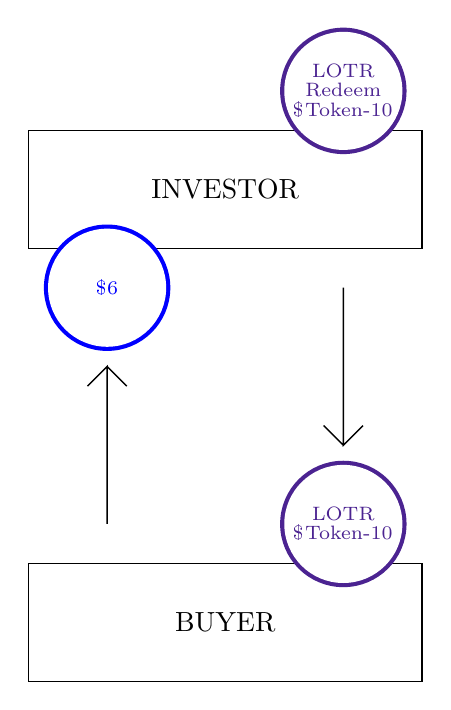
\begin{tikzpicture}
            % bottom box
            \draw [line width=0.5, black] (0,0) -- (5,0) -- (5,1.5) -- (0,1.5) -- (0,0);
            \node [align=center,font=\fontsize{10pt}{10pt}\selectfont] at (2.5,0.75) {BUYER};
            % arrow up
            \draw [line width=0.5, black] (1,2) -- (1,4) -- (0.75,3.75) -- (1,4) -- (1.25,3.75);
            % top box
            \draw [line width=0.5, black] (0,5.5) -- (5,5.5) -- (5,7) -- (0,7) -- (0,5.5);
            \node [align=center,font=\fontsize{10pt}{10pt}\selectfont] at (2.5,6.25) {INVESTOR};
            % STABLECOIN top left
            \draw [line width=3, blue] (1,5) circle (0.75);
            \fill [white,fill opacity=1] (1,5) circle (0.75);
            \node [color=blue,align=center,font=\fontsize{7pt}{7pt}\selectfont] at (1,5) {\$6};
            % Redeem Token
            \draw [line width=3, color={rgb:red,130;green,60;blue,250}] (4,7.5) circle (0.75);
            \fill [white,fill opacity=1] (4,7.5) circle (0.75);
            \node [color={rgb:red,130;green,60;blue,250},align=center,font=\fontsize{7pt}{7pt}\selectfont] at (4,7.5) {LOTR\\Redeem\\\$Token-10};
            % arrow down
            \draw [line width=0.5, black] (4,5) -- (4,3) -- (4.25,3.25) -- (4,3) -- (3.75,3.25);
            % Limit Order Token bottom right
            \draw [line width=3, color={rgb:red,130;green,60;blue,250}] (4,2) circle (0.75);
            \fill [white,fill opacity=1] (4,2) circle (0.75);
            \node [color={rgb:red,130;green,60;blue,250},align=center,font=\fontsize{7pt}{7pt}\selectfont] at (4,2) {LOTR\\\$Token-10};
         \end{tikzpicture}
      \end{center}

      Over time, \$Token loses \$1 in value, now trading for \$11 per token. Because the market price is now closer to the limit order target price, based on the historical volatility of \$Token, the Limit Order token is now valued at \$6 per token. Loss = \$1, Gain = \$2. \\

      The investor does not think \$Token will continue to decrease in value, so they buy back a Redeem Token for \$Token @ \$10, which is now valued at \$4 per token. Expense = \$4.
      % TRADING GRAPHIC
      \begin{center}
         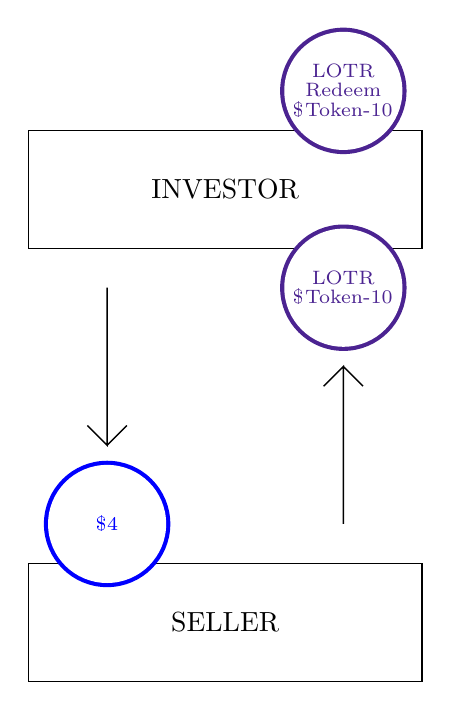
\begin{tikzpicture}
            % bottom box
            \draw [line width=0.5, black] (0,0) -- (5,0) -- (5,1.5) -- (0,1.5) -- (0,0);
            \node [align=center,font=\fontsize{10pt}{10pt}\selectfont] at (2.5,0.75) {SELLER};
            % arrow down
            \draw [line width=0.5, black] (1,5) -- (1,3) -- (.75,3.25) -- (1,3) -- (1.25,3.25);
            % top box
            \draw [line width=0.5, black] (0,5.5) -- (5,5.5) -- (5,7) -- (0,7) -- (0,5.5);
            \node [align=center,font=\fontsize{10pt}{10pt}\selectfont] at (2.5,6.25) {INVESTOR};
            % STABLECOIN
            \draw [line width=3, blue] (1,2) circle (0.75);
            \fill [white,fill opacity=1] (1,2) circle (0.75);
            \node [color=blue,align=center,font=\fontsize{7pt}{7pt}\selectfont] at (1,2) {\$4};
            % Redeem Token
            \draw [line width=3, color={rgb:red,130;green,60;blue,250}] (4,7.5) circle (0.75);
            \fill [white,fill opacity=1] (4,7.5) circle (0.75);
            \node [color={rgb:red,130;green,60;blue,250},align=center,font=\fontsize{7pt}{7pt}\selectfont] at (4,7.5) {LOTR\\Redeem\\\$Token-10};
            % arrow up
            \draw [line width=0.5, black] (4,2) -- (4,4) -- (3.75,3.75) -- (4,4) -- (4.25,3.75);
            % Limit Order Token
            \draw [line width=3, color={rgb:red,130;green,60;blue,250}] (4,5) circle (0.75);
            \fill [white,fill opacity=1] (4,5) circle (0.75);
            \node [color={rgb:red,130;green,60;blue,250},align=center,font=\fontsize{7pt}{7pt}\selectfont] at (4,5) {LOTR\\\$Token-10};
         \end{tikzpicture}
      \end{center}

      The investor redeems the LOTR collateral of \$10. Revenue = \$10.
      % REDEEM GRAPHIC
      \begin{center}
         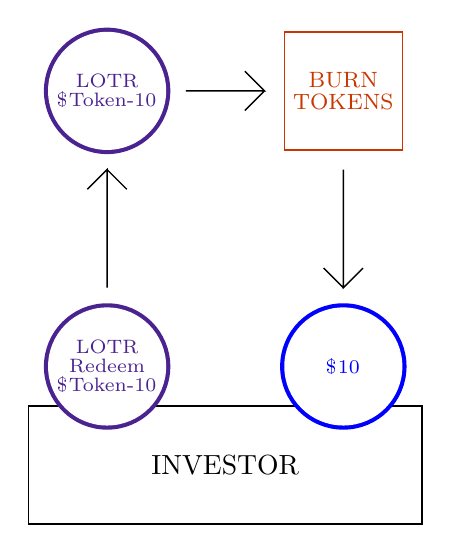
\begin{tikzpicture}
            % bottom box
            \draw [line width=0.5, black] (0,0) -- (5,0) -- (5,1.5) -- (0,1.5) -- (0,0);
            \node [align=center,font=\fontsize{10pt}{10pt}\selectfont] at (2.5,0.75) {INVESTOR};
            % Redeem Token bottom left
            \draw [line width=3, color={rgb:red,130;green,60;blue,250}] (1,2) circle (0.75);
            \fill [white,fill opacity=1] (1,2) circle (0.75);
            \node [color={rgb:red,130;green,60;blue,250},align=center,font=\fontsize{7pt}{7pt}\selectfont] at (1,2) {LOTR\\Redeem\\\$Token-10};
            % arrow up
            \draw [line width=0.5, black] (1,3) -- (1,4.5) -- (0.75,4.25) -- (1,4.5) -- (1.25,4.25);
            % Limit Order Token top left
            \draw [line width=3, color={rgb:red,130;green,60;blue,250}] (1,5.5) circle (0.75);
            \fill [white,fill opacity=1] (1,5.5) circle (0.75);
            \node [color={rgb:red,130;green,60;blue,250},align=center,font=\fontsize{7pt}{7pt}\selectfont] at (1,5.5) {LOTR\\\$Token-10};
            % arrow right
            \draw [line width=0.5, black] (2,5.5) -- (3,5.5) -- (2.75,5.75) -- (3,5.5) -- (2.75,5.25);
            % Burn tokens box
            \draw [line width=0.5, color={rgb:red,255;green,70;blue,0}] (3.25,4.75) -- (3.25,6.25) -- (4.75,6.25) -- (4.75,4.75) -- (3.25,4.75);
            \node [color={rgb:red,255;green,70;blue,0},align=center,font=\fontsize{8pt}{8pt}\selectfont] at (4,5.5) {BURN\\TOKENS};
            % arrow down
            \draw [line width=0.5, black] (4,4.5) -- (4,3) -- (4.25,3.25) -- (4,3) -- (3.75,3.25);
            % STABLECOIN bottom right
            \draw [line width=3, blue] (4,2) circle (0.75);
            \fill [white,fill opacity=1] (4,2) circle (0.75);
            \node [color=blue,align=center,font=\fontsize{7pt}{7pt}\selectfont] at (4,2) {\$10};
         \end{tikzpicture}
      \end{center}
      
      The investor's account net change:
      \begin{tabbing}
         ~~~~ \= $-$ \= \$10 \= ~~~~ \= LOTR mint cost \\
         \> $+$ \>\$6 \> ~~~~ \> sale of Redeem Token \\
         \> $-$ \>\$1 \> ~~~~ \> unrealized loss in \$Token \\
         \> $+$ \>\$2 \> ~~~~ \> value increase of Limit Order token \\
         \> $-$ \>\$4 \> ~~~~ \> repurchase of Redeem Token \\
         \> $+$ \>\$10 \> ~~~~ \> LOTR collateral redemption \\
         ~~~~ \par\noindent\rule{8cm}{0.4pt} \\
         \> $+$ \>\$3 \\
      \end{tabbing}

      Including both unrealized and realized changes, the investor portfolio gains \$3 during this period rather than losing \$1. A different mix of positions using LOTRs at different limit price targets can be used to achieve a delta neutral portfolio, if desired. \\
      
      Please note that fees were not considered in this example, and can create considerable outcome differences depending on the hosting blockchain native token price, high gas limits, and other trading fees.

   \section*{Valuation}
      Note: The discovery of the ideal formula describing the market valuation of LOTR tokens is ongoing. Modeling of the best pricing formula consider the Black-Scholes model and Martingale pricing, among other continuously revised hedging methods in an attempt to find a delta neutral approach to valuation. This valuation methodology assumes a liquid market of regularly spaced LOTR limit tokens with no fees and zero swap slippage. \\

      For now we will consider a generalized valuation model that represents the incomplete portion of the model with a single constant that can be modified according to traders' preferences.

      \subsection*{Limit Orders Below Market Price}
      \begin{center}
      \includegraphics[scale=0.6]{graph_limit_below.png}
      \end{center}
      \begin{center}
      \includegraphics[scale=0.6]{graph_redeem_below.png}
      \end{center}

      \subsection*{Limit Orders Above Market Price}
      Limit Orders above the current market price do not traditionally exist since market makers will automatically fill orders of this type. Typically a Stop Order would be placed first to prevent the broker from issuing the Limit Order to the market maker until the Stop price is reached, but the unique nature of smart contracts allows us to create seamless fungible products, and so we will call these orders simply "Limit Orders" so that the product can be perpetually referenced consistenly regardless of its current internal state.

      \begin{center}
      \includegraphics[scale=0.6]{graph_limit_above.png}
      \end{center}
      \begin{center}
      \includegraphics[scale=0.6]{graph_redeem_above.png}
      \end{center}

\end{document}